\documentclass[parskip=full]{scrartcl}
\usepackage[utf8]{inputenc} % use utf8 file encoding for TeX sources
\usepackage[T1]{fontenc}    % avoid garbled Unicode text in pdf
\usepackage[german]{babel}  % german hyphenation, quotes, etc
\usepackage{hyperref}       % detailed hyperlink/pdf configuration
\hypersetup{                % ‘texdoc hyperref‘ for options
	pdftitle={Entwurf},%
	bookmarks=true,%
}
\usepackage{graphicx}       % provides commands for including figures
\usepackage{csquotes}       % provides \enquote{} macro for "quotes"
\usepackage{scrpage2}
\usepackage{caption}
\usepackage{enumitem}
\pagestyle{scrheadings}
\usepackage{float}

%\clearscrheadfoot
\ohead{BPTI: Gruppe 03=\{Niklas Metz, Felix Bachmann\}, Entwurf, WS 2017/18}

\begin{document}
	\section{Idee}
		Unsere Idee besteht darin, ein Bomberman-Spiel zu implementieren. Inspiriert wurden wir durch das Spielprinzip des gleichnamigen Titels von Hudson Soft, herausgegeben 1983 von Nintendo. In unserer Version fokussieren wir uns vorerst auf den Mehrspieler-Modus. 
		Jeder Spieler hat eine Bombe, die er auf freien Felder platzieren kann. Diese explodiert nach einer gewissen Zeit, woraufhin die Bombe wieder für den Spieler zur Verfügung steht.
		Das Spielziel besteht darin, den Gegenspieler durch das strategische Platzieren von Bomben auszuschalten. \newline
		Hierbei wird in einer Arena gespielt, die nach außen hin durch unzerstörbare Blöcke abgegrenzt ist. Im Inneren der Arena existieren sowohl durch Bomben zerstörbare Blöcke als auch unzerstörbare Blöcke. Die unzerstörbaren Blöcke dienen zum Schutz der Spieler vor Explosionen. \newline
		Jeder Spieler hat eine gewisse Anzahl an Leben. Das Spiel ist beendet, wenn nur noch ein Spieler Leben übrig hat.
		\begin{figure}[H]
			\centering
			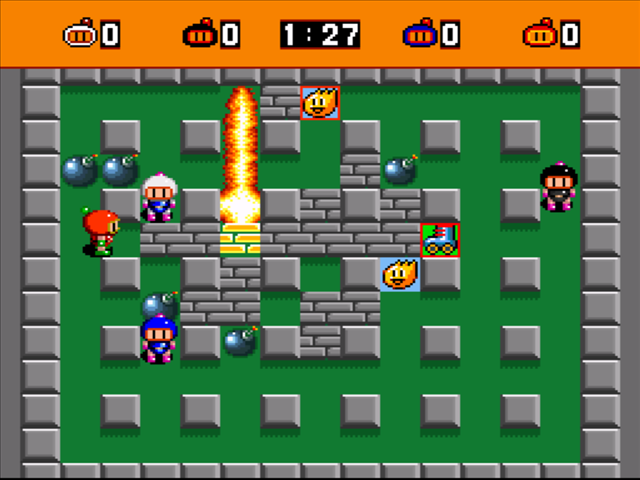
\includegraphics[scale=0.6]{../bomberman.png}
			\centering
			\caption*{Super Bomberman, SNES \newline Quelle: \url{http://hero.wikia.com/wiki/File:Super-bomberman-1-02.png} }
		\end{figure}
		
	
	\section{Ziele}
		\subsection{Musskriterien}
			\subsubsection{Darstellung}
				\begin{itemize}[noitemsep]
					\item zwei rechteckige Spielfiguren (einfarbig)
					\item zwei verschiedene Block-Arten (einfarbig)
					\item Explosionen (einfarbig)
					\item tickende Bomben (Farbwechsel)
				\end{itemize}
				
			\subsubsection{Benutzer-Interaktion}
				\begin{itemize}[noitemsep]
					\item Bewegung der zwei Spielfiguren durch ein Eingabegerät
					\item Platzieren von Bomben
				\end{itemize}
				
			\subsubsection{Spielmechanik}
				\begin{itemize}[noitemsep]
					\item Start eines neuen Spieldurchgangs (durch Reset-Knopf und bei Spielstart automatisch)
					\item Spielfiguren können sich nicht durch Blöcke hindurch bewegen
					\item Bomben explodieren nach einer gewissen Zeit
					\item zerstörbare Blöcke verschwinden nach einer Explosion, die sich an einem angrenzenden Feld des Blockes ereignet
					\item unzerstörbare Blöcke werden von einer angrenzenden Explosion nicht beeinflusst
					\item Spielfiguren, die sich in einer Explosion befinden, verschwinden und verlieren das Spiel
				\end{itemize}
		
		\subsection{Wunschkriterien}
			\subsubsection{Darstellung}
			\begin{itemize}[noitemsep]
				\item Sprites für Spielfiguren, Bomben, Explosionen, Blöcke und Powerups 
				\item Status-Anzeige (Leben, Anzahl Bomben etc.)
				\item Titelbildschirm
			\end{itemize}
			
			\subsubsection{Spielmechanik}
			\begin{itemize}[noitemsep]
				\item verschiedene zufällig platzierte Powerups (Erhöhung der Bomben-Anzahl etc.)
				\item mehrere Leben pro Spieler
				\item automatischer Neustart nach Spielende
				\item bis zu vier Spieler
				\item KI-Gegner zum Auffüllen der vier Spieler
			\end{itemize}
	\newpage
	\section{Projektplan}
		Wir haben uns dazu entschieden den Schaltungsentwurf, sowie die Test-Phase nicht einer einzelnen Person zuzuteilen. \newline
		Der Schaltungsentwurf ist für den weiteren Verlauf des Projektes richtungsweisend, da der logische Aufbau des Systems maßgeblich für die Implementierung der einzelnen Komponenten ist. \newline
		In der Test-Phase wird das Gesamtsystem, also die Verschaltung der Unterkomponenten, auf Korrektheit überprüft und gegebenenfalls erweitert. Da hierfür eine direkte Kommunikation der Implementierenden erforderlich ist, entschieden wir uns dazu die Phase gemeinsam durchzuführen.
		
		\begin{table}[H]
			\centering
			\label{my-label}
			\begin{tabular}{l|l|l}
				Ziel                                      & Verantworliche(r) & Zeitvorgabe  \\
				\hline
				Schaltungsentwurf                         & beide           & bis 15.12.17 \\
				Darstellung des Spielfelds                & Niklas          & bis 22.12.17 \\
				Blockverteilung auf Spielfeld             & Felix           & bis 22.12.17 \\
				Spielfigur - Darstellen, Bewegen          & Felix           & bis 08.01.18 \\
				Spielfigur - Kollision                    & Niklas          & bis 15.01.18 \\
				Platzieren von Bomben                     & Niklas          & bis 15.01.18 \\
				Ticken der Bombe                          & Felix           & bis 18.01.18 \\
				Explosionen - Darstellung                 & Niklas          & bis 26.01.18 \\
				Explosionen - Kollision (Spieler, Blöcke) & Felix           & bis 01.02.18 \\
				Testen, Debugging, Wunschkriterien        & beide           & bis 08.02.18
			\end{tabular}
		\end{table}

				
\end{document}